\documentclass[11pt,a4paper]{article}
% \documentclass[a4paper]{article}
% \usepackage[brazil]{babel} % carrega portugues brasileiro
\usepackage[utf8]{inputenc}
\usepackage[T1]{fontenc}
\usepackage[top=2cm, bottom=2cm, left=2cm, right=2cm]{geometry} %margens menores!
\usepackage{graphicx} % incluir figuras .eps
\usepackage{tabularx}
\usepackage{color} % colorir texto
\usepackage{indentfirst}
\usepackage{textcomp}
\usepackage[colorlinks=true]{hyperref}
\usepackage{amssymb,amsmath}
\usepackage{float}
\usepackage{wrapfig}
% \usepackage{siunitx}
% \usepackage[ampersand]{easylist}

\title{User Manual}


\author{
       \large
       \mbox{Rhizomatica} \\
       \mbox{}\\ 
       \textsc{Rafael Diniz}
        rafael@rhizomatica.org\\
%        \normalsize
%        we want the airwaves
%        \texttt{Brasília - Brasil}\\
}
\date{\today}

\begin{document}

\maketitle

\begin{figure*}[!ht]

\includegraphics[width=1\textwidth]{pictures/logoh.png}
\end{figure*}

\begin{abstract}

This is the user manual of the High-Frequency Emergency and Rural Multimedia Exchange System (HERMES) digital telecommunication system. HERMES combines a set of technologies in order to provide telecommunications services over the HF frequency band. Among these technologies are an affordable HF transceiver, a high-performance software-defined modem, the Unix-to-Unix Communication Protocol (UUCP) and a set of carefully configured user services which are available over a local WiFi network. This manual addresses the basic equipment operation, including the usage of the web-based graphic user interface (GUI) and the email transport system.

\end{abstract}

\newpage

\tableofcontents

\setlength{\parindent}{0em}
\setlength{\parskip}{1em}

\section{Introduction}

HERMES is a telecommunication system which operates in the High Frequency (HF) band. HERMES allows digital multimedia exchange between users and stations, including exchange of text, image, audio or any other file type. The system interface to the users is a web interface available to users within WiFi connectivity distance to a HERMES transceiver.  

The system relies heavily on the e-mail protocol, which can be managed and accessed thought the system's web interface or through specialized apps, like DeltaChat\footnote{DeltChat, a multi-plataform e-mail messenger: \url{https://delta.chat/} }. HERMES also supports peer-to-peer secure messages between the Host stations, which works as a bulletin board system (BBS).

The system employs a star topology network in which a Gateway station connects to all Host stations in remote locations. The Gateway station routes e-mail and other messages locally (back to Host stations over HF) or over the Internet to the wider world. The synchronization between the data to be sent or received from each remote station is asynchronous and orchestrated by the Gateway station in a round-robin fashion (one Host station after another, in order) during pre-established times.

\begin{figure*}[!ht]
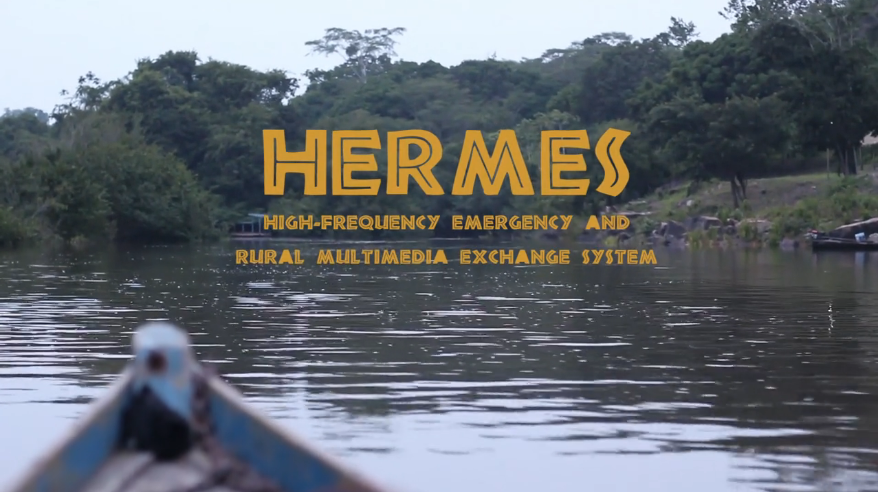
\includegraphics[width=1\textwidth]{pictures/hermes.png}
\end{figure*}

\subsection{HERMES HF Transceiver}

The front panel of the equipment is shown in Figure~\ref{fig:frontview}.

The HERMES box includes the following input / output interfaces, as shown in Figure~\ref{fig:backview}.

\begin{enumerate}
    \item Back Panel - Serial number;
    \item Back Panel - Ground connector;
    \item Back Panel - Ventilation openings;
    \item Back Panel - HF antenna connector (PL-259 / UHF female);
     \item Back Panel - Fuse (10A);
     %fuse number
    \item Back Panel - 12V DC power input, positive (red) and negative (black) terminals;
    \item Back Panel - WiFi antenna connector (RP-SMA female);
    \item Back Panel - RJ-45 Ethernet port, for connection to external switch or router;
    \item Front Panel - Power switch (on/off);
    \item Front Panel - 4 indicator LED's (System LED, Antenna Status LED, Connected LED, TX LED).
\end{enumerate}

\begin{figure}[!ht]
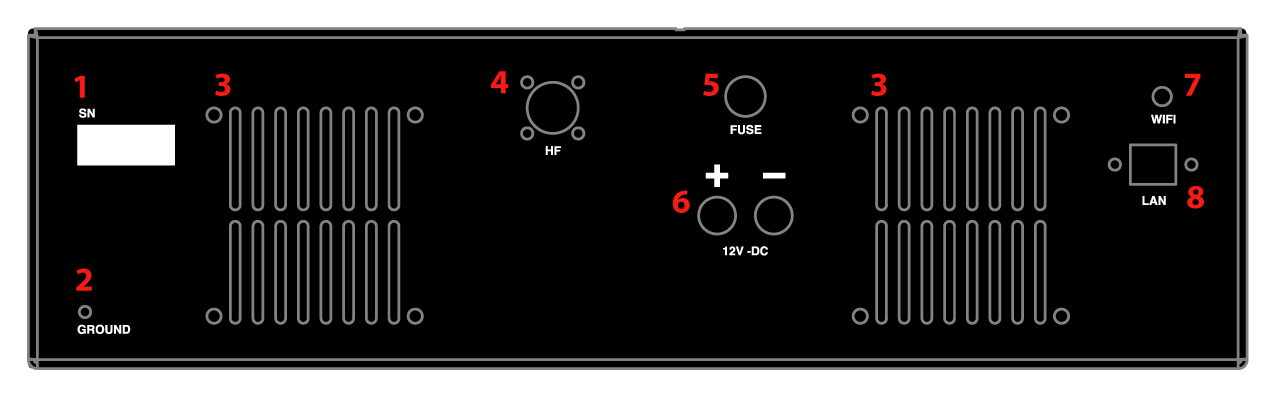
\includegraphics[width=1\textwidth]{pictures/traseiro.png}
\caption{Back view of HERMES box}
\label{fig:backview}
\end{figure}

\begin{figure}[!ht]
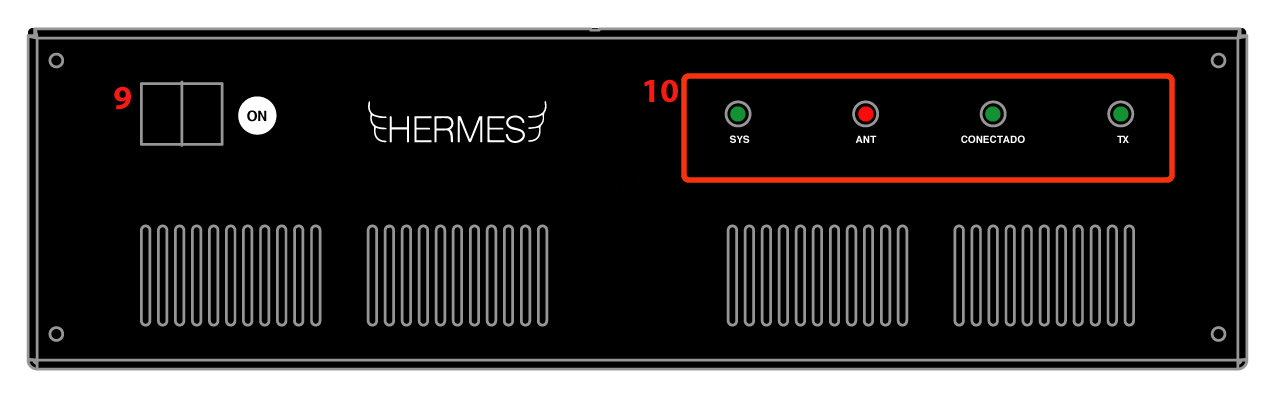
\includegraphics[width=1\textwidth]{pictures/front.png}
\caption{Indicator's LED on front panel}
\label{fig:frontview}
\end{figure}
The LED indicator lights are set to show the following:
\begin{itemize}
    \item SYS: System LED, blinks when the system is not ready to be used. SYS LED typically blinks when the equipment is turning on or when it is turning off;
    \item ANT: Green when the antenna is functioning properly, and no high SWR value is detected. ANT LED turns Red when a high SWR value is detected, meaning the high SWR protection is enabled and the radio will not transmit. SWR protection needs to be reset if active (Red), for the radio to became operational again, which can be done in the radio administrative interface. Check the RF cable and Antenna before resetting in the interface;
    \item CONECTADO: LED on (solid Green) means that the station is connected to another station;
    \item TX: LED on means the radio is transmitting. When this LED is off, it is in receive mode. If the CONECTADO LED is on and the TX LED is off, the station is actively receiving. During active communication with another station the CONECTADO LED will be solid Green and the TX LED will turn on and off;
\end{itemize}


\subsection{HF Antenna Recommendation}

An HF antenna tuned to the desired operating frequency must be connected to the equipment. Never turn on the equipment without first connecting to an appropriate antenna!

There are many HF antennas, each one fitting a different purpose. For short and medium range communications (up to about 800 km), a quarter wavelength dipole installed in inverted V configuration is a good and affordable option. %could include a link to the Rhizomatica HF manual here. 

\subsection{Power Requirements}

The system is designed to operate with between 12V DC to 14V DC power. A typical setup would use 12V DC from a battery connected to a solar charge controller and photo-voltaic panels. Another setup option is to use a 12V or 13.8V AC/DC power supply. 

The red connector on the back of the transceiver should be connected to the positive (+) polarity of the battery or power supply unit, while the black connector to the negative (-) polarity. The system has polarity inversion protection, but care should be taken to proper power installation of power connections. The transceiver consumes approximately 2A in receive mode, and 6A in transmit mode. %is receive mode the same thing as standby?

\section{Web Interface}

HERMES provides a web interface which can be accessed through a local WiFi network. When accessing the HERMES WiFi network, the following information applies:
\begin{itemize}
    \item Network Name (ESSID): HERMES
    \item Password: amazonia
\end{itemize}

Be aware that on some mobile phones a browser will automatically open with the the main HERMES web page, while in others, to access the HERMES web interface, you must open the browser and access \url{http://ac1.hermes.radio} or \url{http://10.0.0.1}. 
\linebreak
\linebreak
O navegador chrome / chromium é o navegador padrão para utilização da interface HERMES, para garantir uma melhor experiência faça preferência pelos navegadores informados.

\begin{figure}[H]
    \centering
    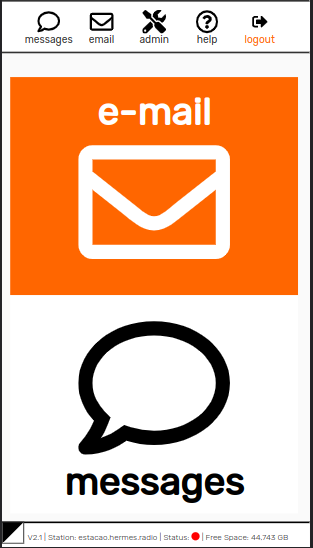
\includegraphics[width=0.5\columnwidth]{screenshots/frontend/en/landing.png}
    \caption{Hermes home}
    \label{fig:messagesindex}
\end{figure}

\begin{figure}[H]
    \centering
    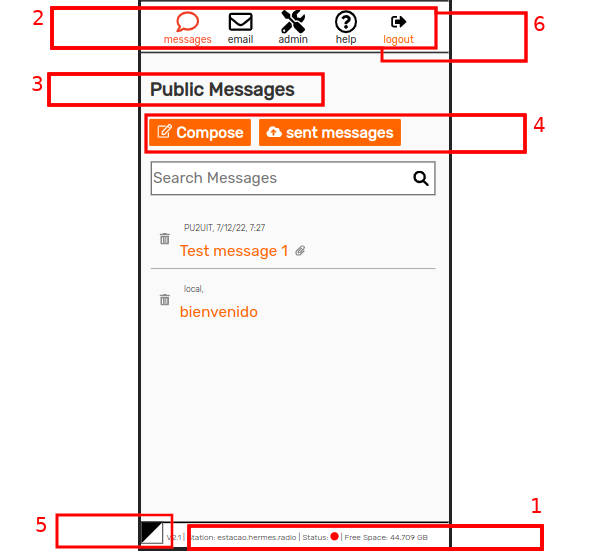
\includegraphics[width=1\columnwidth]{screenshots/frontend/en/messagesindex_enUS.png}
    \caption{Hermes public messages and elements}
    \label{fig:messagesindex}
\end{figure}
    
On the public messages page \ref{fig:messagesindex} you will find the following links:

\begin{enumerate}
    \item Station information and status;
    \item Main menu;
    \item Welcome message (page title);
    \item Link to sent messages and new message;
    \item Dark/light mode activator tab;
    \item Login and logout link and info;
\end{enumerate}

\begin{figure}[H]
    \centering
    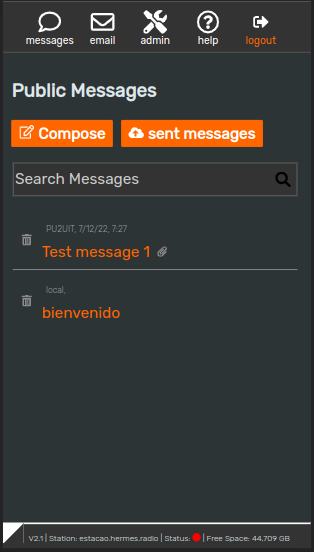
\includegraphics[width=0.5\columnwidth]{screenshots/frontend/en/darkmode.png}
    \caption{Hermes Dark Mode}
    \label{fig:darkmode}
\end{figure}
    
The web interface allows admin users to manage e-mail accounts, to perform radio configurations (like setting frequency and SSB mode) and exchange direct messages between stations (BBS). The interface also contains its own administrative section, for defining and managing users and their privileges. 

It is important to note that same user name created for the administrative interface will be used for the e-mail address assigned to that user.  For example, user "amelia" in the local interface will have the email "amelia@ac2.hermes.radio". Note that the email address is composed of the user name @ the name of the station, which corresponds to its internet domain name, in this example, "ac2.hermes.radio". Each station domain name is written in the header on the Hermes web interface. If the domain begins with "ga" then it is a Gateway station.

\subsection{Administrative Interface}
\label{admininterface}

\begin{figure}[H]
    \centering
    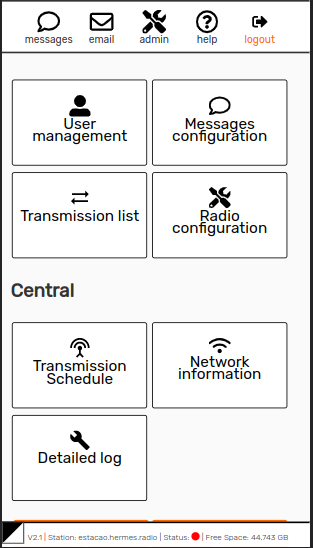
\includegraphics[width=0.5\columnwidth]{screenshots/frontend/en/admin.png}
    \caption{Admin interface}
    \label{fig:admin}
\end{figure}

To access admin features, you need an admin password. While anyone can create a user account, only a system admin can create new administrator user and give admin power to other users. To login, click on the login icon on the top right of the web interface. 

The default administrator login username is: "root" and the password is: "caduceu".

Inside the administration section, an admin user will find the following options: user management, messages administration, network information, stations, detailed log and radio configuration.

\subsubsection{User management} 

Allows the creation of new users, updating data of registered users and to delete users of the system. Every username corresponds to an email account with the same name as in the example above (e.g. amelia@ac2.hermes.radio). 
    
    \begin{figure}[H]
    \centering
    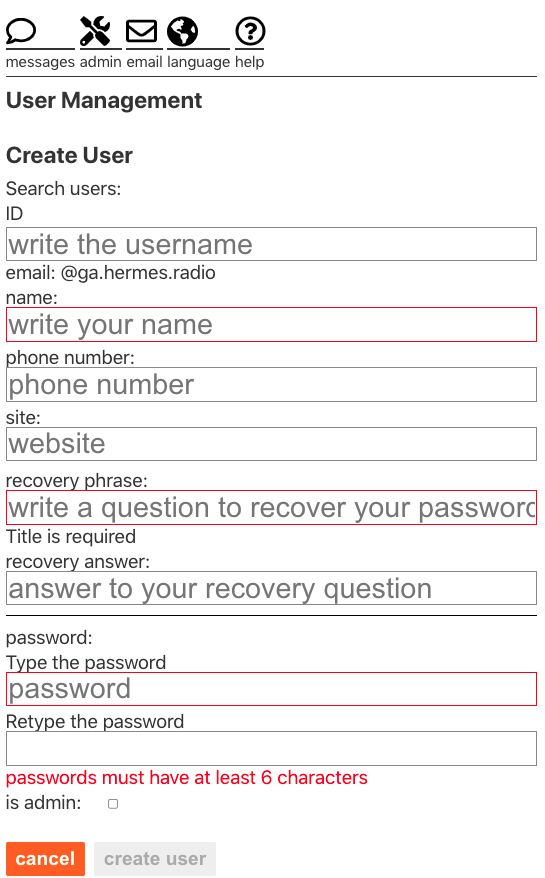
\includegraphics[width=0.5\columnwidth]{screenshots/frontend/en/createuser.png}
    \caption{Create user interface}
    \label{fig:createuser}
    \end{figure}
    
    Administrators can also give admin powers to regular users, by clicking on the "is admin" checkbox at the bottom of the Create User page.

\subsubsection{Messages administration}  
\label{gui_msg_admin}

From this page, an admin can determine who will be able to send public messages between stations and who can attach files to this messages: everyone; only registered users or only administrators. It is worth thinking this through with the users as attachments can slow the system down considerably.
   
    \begin{figure}[H]
    \centering
    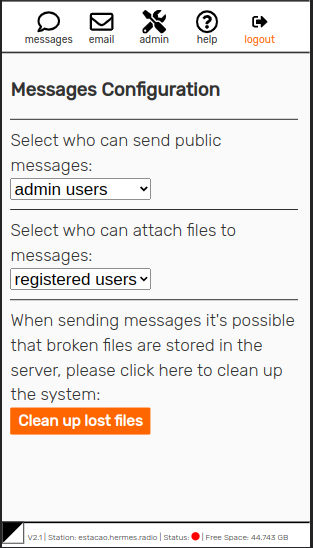
\includegraphics[width=0.5\columnwidth]{screenshots/frontend/en/messageadm.png}
    \caption{Messages administration Interface}
    \label{fig:messageadm}
   
    \end{figure}


\subsection{Transmission List}
\label{gui_trans_list}

All data exchange in the HERMES system is done through UUCP. Being an asynchronous protocol, all the data is first queued before being transmitted. The elements of the UUCP queue are called "jobs", and each job in the HERMES system can be an e-mail, a public message, or special remote command execution message (for example, to inform of a new e-mail user creation). A system administrator can cancel a job before it is sent. Administrators can also erase the public messages for any reason, including the case when the equipment storage space is reaching its limit. The storage space available is shown in the web interface footer.

The queues of all Host stations are transmitted periodically when the Gateway station connects to each remote station based on whatever schedule has been configured. In an emergency, a system administrator can force message transmission and bypass the queue by clicking on the "force" link. This could interrupt receiving messages from other stations for a while and should be avoided unless absolutely necessary.   
    \begin{figure}[H]
    \centering
    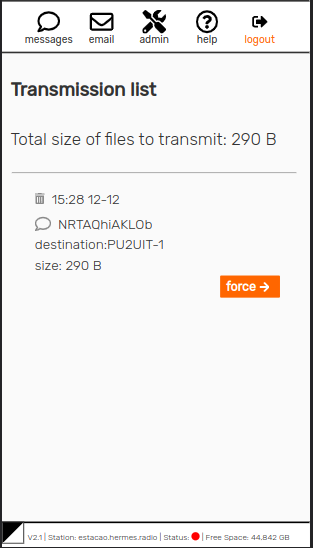
\includegraphics[width=0.5\columnwidth]{screenshots/frontend/en/transmission.png}
    \caption{Transmission list interface}
    \label{fig:transmission}
   
    \end{figure}    
    
    
\subsubsection{Radio configuration}
\label{gui_radio_config}

Provides a direct interface to change various radio settings like frequency, transmission mode, restore factory configuration and it also allows one to view sensor readings about the HF antenna of the system. %we should provide more in-depth information about what the values mean, what to be careful about changing, etc.

\begin{figure}[H]
    \centering
    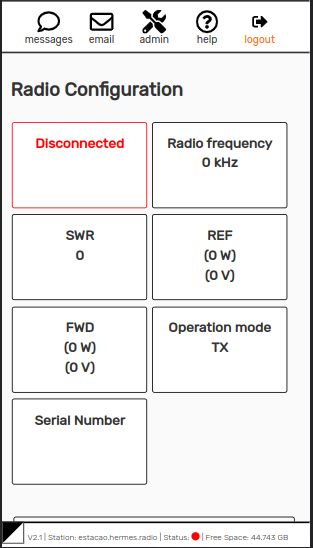
\includegraphics[width=0.5\textwidth]{screenshots/frontend/en/radioconfig.png}
    \caption{Radio configuration interface}
	\vspace{-10pt}
    \label{fig:radioconf}
\end{figure}    

\begin{figure}[H]
    \centering
    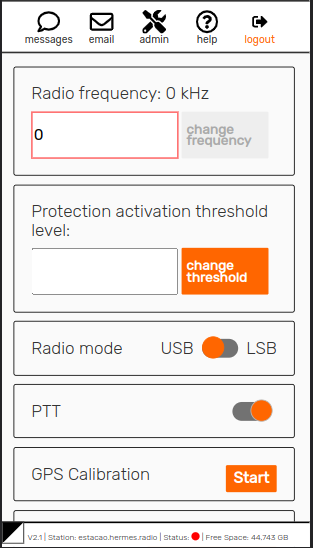
\includegraphics[width=0.5\textwidth]{screenshots/frontend/en/radioconfig2.png}
    \caption{Radio configuration interface}
	\vspace{-10pt}
    \label{fig:radioconf2}
\end{figure}

\subsubsection{Central Station} 
\label{gui_central_station}

The central station is a special station that keeps connected to the internet. If you are in the central station, this option will be shown in the menu. From there is possible to create schedules for transmission to other stations, that are the time slots when the transmission will happen between all the stations connected to the network. It's possible also to enable or disable schedules or change their times from this menu.

\begin{figure}[H]
    \centering
    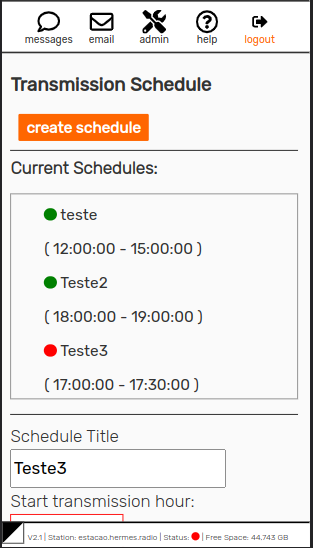
\includegraphics[width=0.5\textwidth]{screenshots/frontend/en/central.png}
    \caption{Transmission schedule}
	\vspace{-10pt}
    \label{fig:central}
\end{figure} 

\begin{figure}[H]
    \centering
    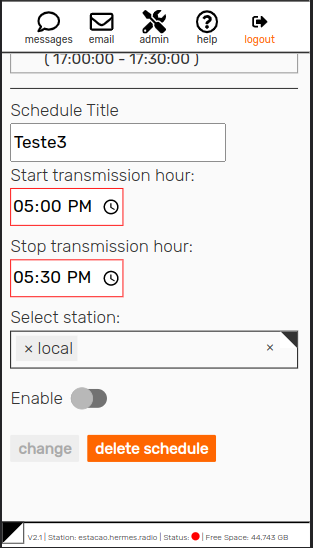
\includegraphics[width=0.5\textwidth]{screenshots/frontend/en/central2.png}
    \caption{Transmission schedule}
	\vspace{-10pt}
    \label{fig:central2}
\end{figure} 


\subsubsection{Network info} 
\label{gui_net_info}

Displays some information about the system, such as network addresses, callsign, servername etc
     \begin{figure}[H]
     \vspace{-10pt}
    \centering
    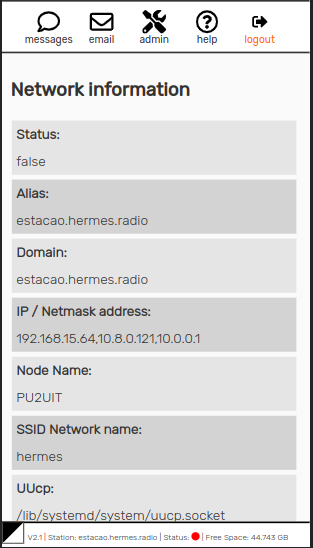
\includegraphics[width=0.5\columnwidth]{screenshots/frontend/en/networkinfo.png}
    \caption{Network information page}
    \label{fig:netinfo}
  
    \end{figure}
    
\subsubsection{Stations} 
\label{gui_stations}

Provides a list of the available stations on the system. 
% If the station is a gateway station, you can choose which stations will be enabled to transmit and receive messages.

\begin{figure}[H]
    \centering
    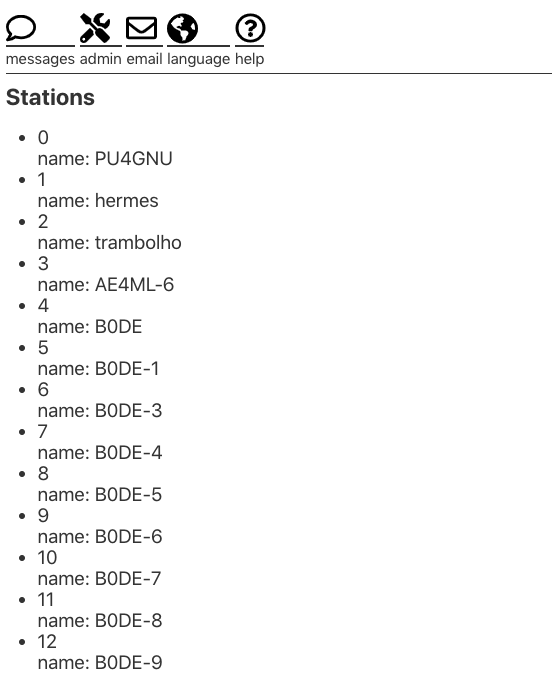
\includegraphics[width=0.5\textwidth]{screenshots/frontend/en/stations.png}
    \caption{Stations interface}
	\vspace{-10pt}
    \label{fig:stations}
\end{figure} 
 


    
\subsubsection{Detailed Log}
Provides access to system logs, such as email logs and UUCP logs, that register every activity on the system.
    
    \begin{figure}[H]
    \centering
    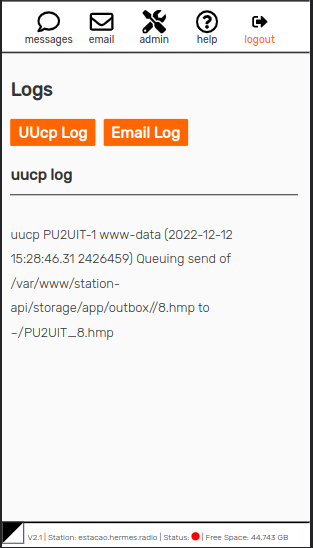
\includegraphics[width=0.5\columnwidth]{screenshots/frontend/en/logs.png}
    \caption{Logs page on the web interface}
    \label{fig:logs}
\end{figure}



\subsection{Public Messages  (BBS)}

Direct messages can be sent between stations with support for cryptography and multimedia compression. Sent and received messages can be found in the Messages tab of the web interface. One Admin of the system can select who will be able to send public messages to other or tho it's own station.

\subsubsection{How to write public messages}


\begin{figure}[H]
    \centering
    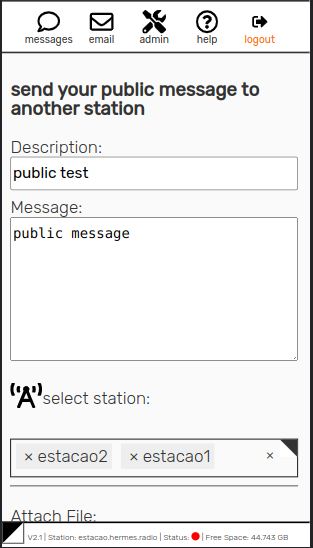
\includegraphics[width=0.5\textwidth]{screenshots/frontend/en/publicas.png}
    \caption{Interface to compose messages}
    \label{fig:compose}
\end{figure}

\begin{figure}[H]
    \centering
    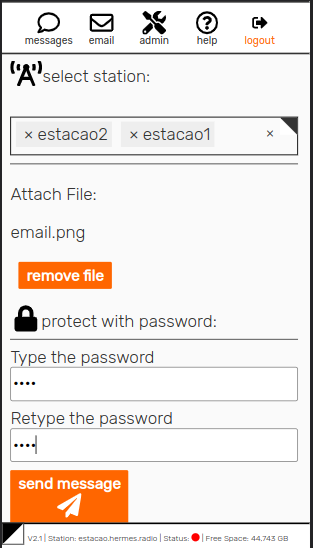
\includegraphics[width=0.5\textwidth]{screenshots/frontend/en/publicas2.png}
    \caption{Interface to compose messages}
    \label{fig:compose}
\end{figure}

By clicking on the compose (
\includegraphics[height=0.8\baselineskip]{pictures/edit.png})icon, it's possible to write a new message and to attach files such as images or audio files. The icon will only show up if it's allowed for the user to compose messages on the station. An admin can determine who can send public messages between stations and who can attach files to public messages by setting permissions in the admin tab. 

Public messages can also be sent to your own station, which is an easy way to publicize news inside your own community.

Public messages can also be password protected, which means that only recipients that know the password will be able to read their content, while the message description will still be readable by everyone. Have in mind that once a password for the message (has to be at least 4 characters) is defined, there is no way to recover it, nor to change it.

On the message administration link in the admin section, a system administrator can change who can attach files to messages between stations: everyone with access to the network, only registered users, or only administrators. 

Because the data throughput over HF is relatively low, file attachments are limited to 20KB. The system will accept inputs for image and sound up to 30 MB and for other files up to 2 MB, and will try to compress them to fit the maximum size of 20KB using state-of-the-art compression techniques. Obviously, this can have an effect on both image and sound file quality. For other file formats, a simple compressor will be applied, and messages with attachment size greater than 20 KB will be cancelled.%does this mean that if you try to send a file larger than 20KB it will automatically cancel, or does it mean that if the compression happens and it is unable to get under 20KB it will cancel?



\subsection{Languages supported}
\label{langs}

The HERMES interface is also available in Portuguese and Spanish, and these versions can be accessed on the Language tab of the main menu.

\begin{figure}[H]
    \centering
    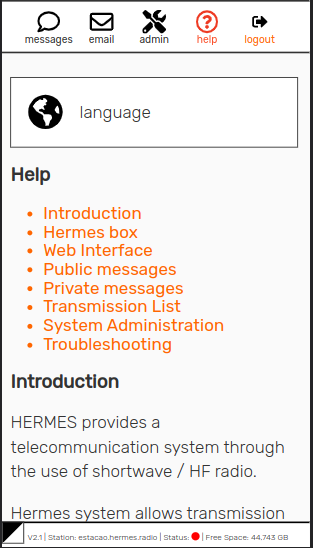
\includegraphics[width=0.5\textwidth]{screenshots/frontend/en/languages.png}
    \caption{Page to access translations}
	\vspace{-10pt}
    \label{fig:languages}
\end{figure}

\begin{figure}[H]
    \centering
    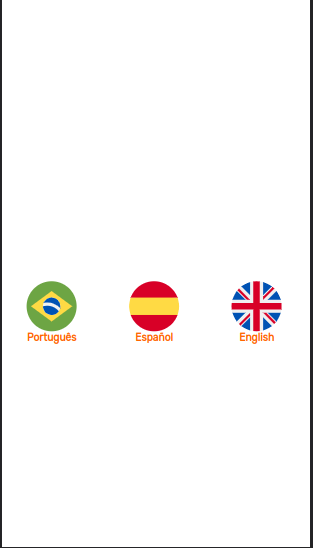
\includegraphics[width=0.5\textwidth]{screenshots/frontend/en/languages2.png}
    \caption{Page to access translations}
	\vspace{-10pt}
    \label{fig:languages2}
\end{figure}

\section{E-mail}
\label{email}

\begin{figure}[H]
    \centering
    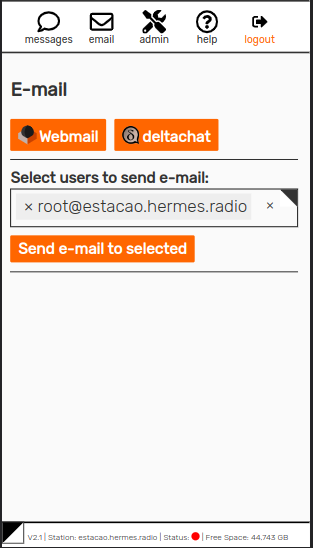
\includegraphics[width=0.5\columnwidth]{screenshots/frontend/en/email.png}
    	\caption{Page to access webmail interface}
	\vspace{-10pt}
    \label{fig:webmail2}
\end{figure}

A key service provided by the HERMES is E-mail. The E-mail is communication protocol attributes to each e-mail bearer an address in the format "username@host". In the case of HERMES, the "username" part of the email is created by a HERMES user in the web interface, while the host (also called domain) is already set in the system, and typically has the format "community\_id.hermes.radio". So a typical HERMES emails looks like, for example, "amelia@ac4.hermes.radio". The "username" is the same username as created in the user creation page in the HERMES administration interface.

HERMES email users can send and receive e-mail just like any other e-mail user. The only restriction which must be considered is that in order to avoid clogging the system with large messages, emails with large attachments will be cancelled by the system, with the appropriate cancellation message sent to the user. %how large? will some compression be applied like with public messages?

While there are many e-mail clients, like Thunderbird and Outlook Express, the recommended e-mail client to be used with HERMES is DeltaChat. DeltaChat installers are available for download through the interface for Android, Windows, MacOS and Linux. A backup option is to use RoundCube webmail which is also accessible through the HERMES web interface.

\subsection{DeltaChat }

\begin{figure}[H]
    \centering
    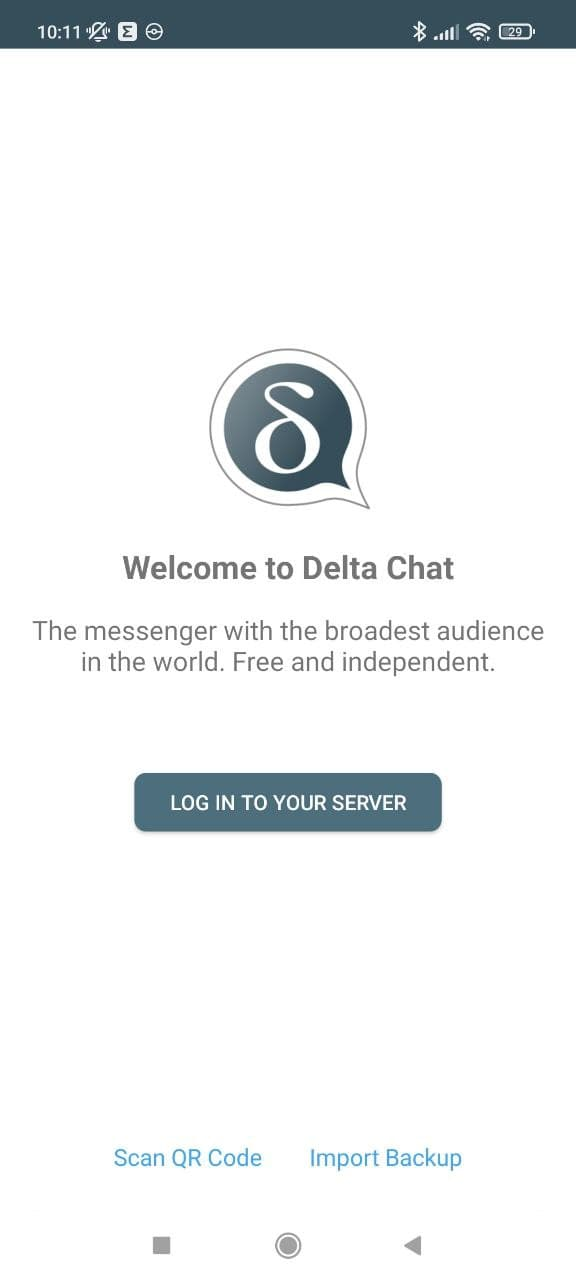
\includegraphics[width=0.3\columnwidth]{screenshots/deltachat/en/intro.jpg}
    	\caption{Deltachat intro (first screen)}
	\vspace{-10pt}
    \label{fig:deltachat-intro}
\end{figure}

\begin{figure}[H]
    \centering
    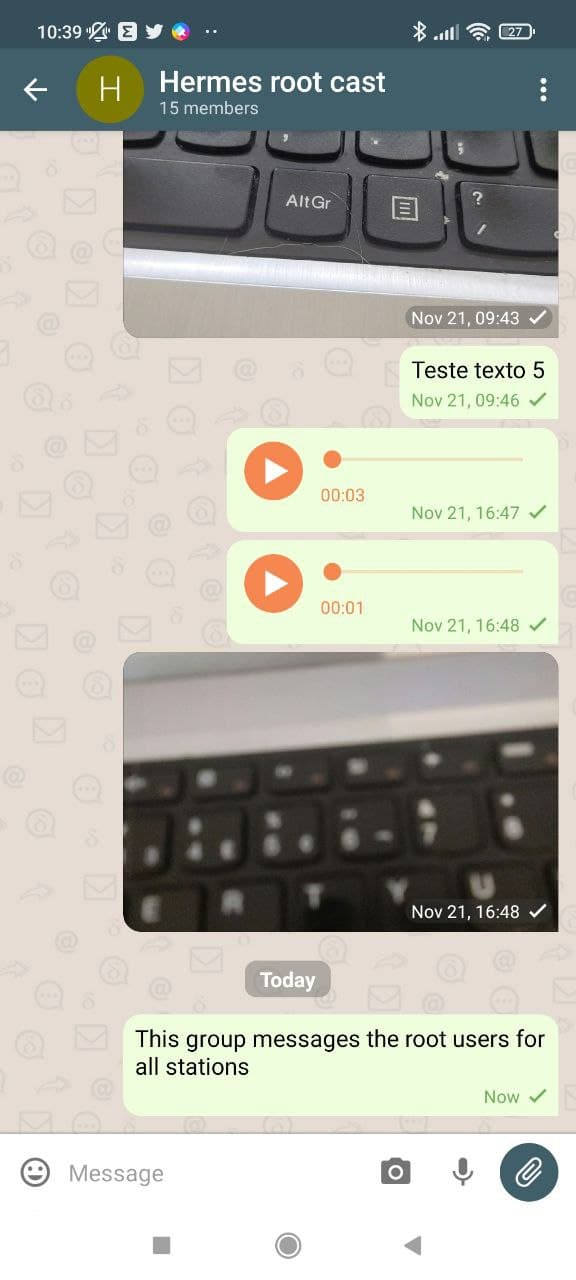
\includegraphics[width=0.3\columnwidth]{screenshots/deltachat/en/chatroom.jpg}
    	\caption{Deltachat chat room example}
	\vspace{-10pt}
    \label{fig:deltachat-chatroom}
\end{figure}

With the DeltaChat application, you can use HERMES email to carry out personal communications for exchanging messages. This app works on most common smartphones and feels like a common messaging application like Telegram, WhatsApp or Signal. Keep in mind that due to the message transmission schedule, messages may take a while to arrive, depending on the amount of messages in the queue and the transmission window length.

\subsubsection{Installation}

DeltaChat is available in most common app stores and repositories. As HERMES is designed for places with low or no connectivity, it is possible to download it through the HERMES web interface, selecting one of the packages provided according to your device operational system. HERMES provides installation files for mobile or computer systems such as Android, GNU/Linux, Windows and MacOSX. The installer files can be accessed here if you're reading this using a HERMES system network: \href{ http://10.0.0.1/dowloads/deltachat.apk}{Android},  \href{ http://10.0.0.1/dowloads/deltachat.exe}{Windows},  \href{ http://10.0.0.1/dowloads/deltachat.deb}{Debian} and \href{http://10.0.0.1/dowloads/deltachat.dmg}{Mac OS}

% FEITO qual endpoint do frontend?

\subsubsection{Configuration}

The HERMES system includes a compression system suitable for multimedia messages like images or audio being sent over HF.  End-to-end encryption should be disabled in order to allow the server-based image and audio compression to work properly, otherwise image and audio exchange will not be possible.

The steps to find this feature in Deltachat are: Burger Menu (
\includegraphics[height=0.78\baselineskip]{pictures/burger.png}) -> Settings -> Advanced -> Autocrypt, turn off: Prefer End-To-End Encryption) as shown in Figure~\ref{fig:deltachat-adv_p2pe}.

\begin{figure}[H]
    \centering
    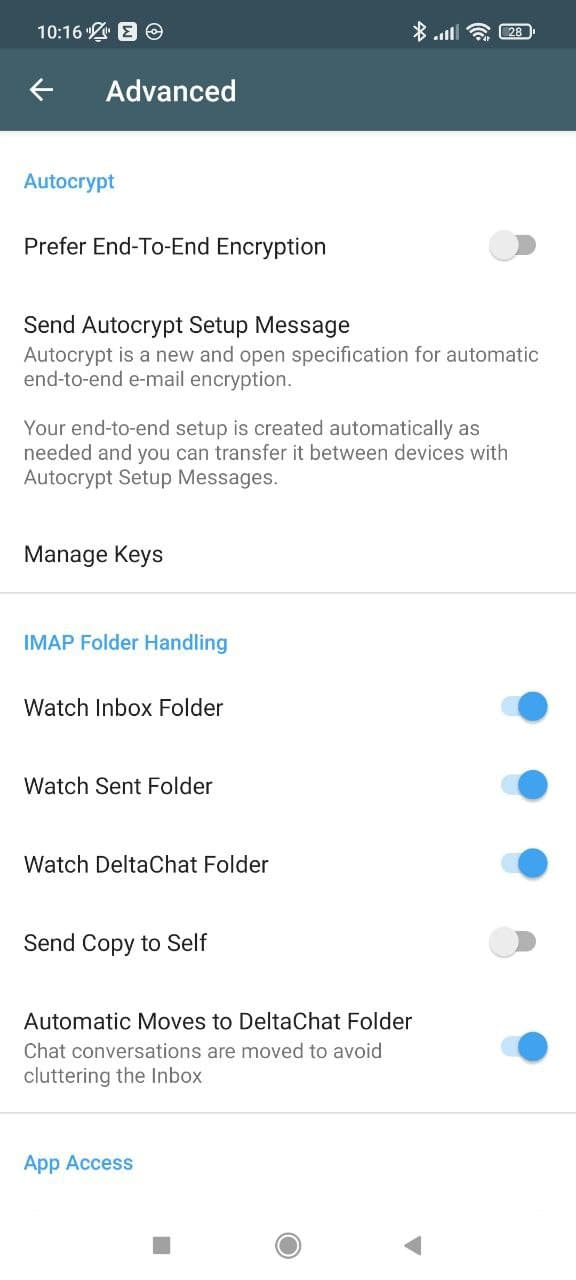
\includegraphics[width=0.3\columnwidth]{screenshots/deltachat/en/adv_p2pe.jpg}
    	\caption{Deltachat Advanced settings}
	\vspace{-10pt}
    \label{fig:deltachat-adv_p2pe}
\end{figure}

Deltachat, by default, tags its emails and show only the "known" messages (emails) that was sent by another Deltachat application. In order to be able to interact with e-mails from any e-mail client software, enable the option "show all emails".
The steps to find this feature in Deltachat are:  Burger Menu (
\includegraphics[height=0.78\baselineskip]{pictures/burger.png}) -> Settings -> Chats and Media -> Show Classic E-Mails -> All. As shown in Figure~\ref{fig:deltachat-allemails}

\begin{figure}[H]
    \centering
    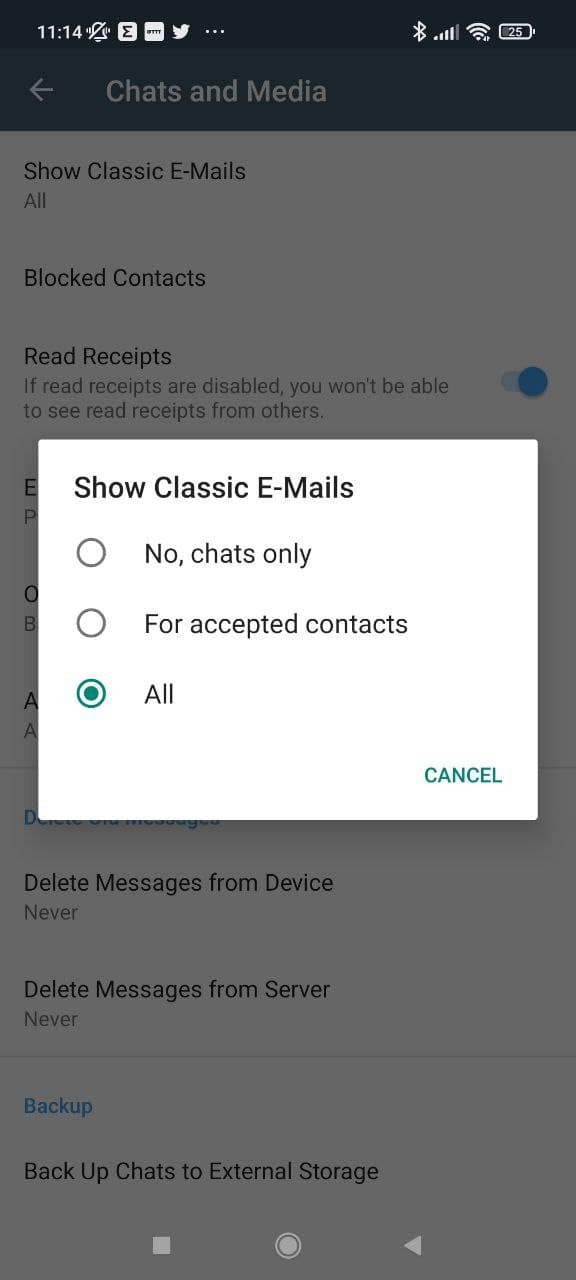
\includegraphics[width=0.3\columnwidth]{screenshots/deltachat/en/allemails.jpg}
    	\caption{Deltachat Setup all emails}
	\vspace{-10pt}
    \label{fig:deltachat-allemails}
\end{figure}

\subsubsection{Usage}

In order to configure DeltaChat, first an e-mail account should be created, as described in section~\ref{admininterface}. In order to login to an e-mail account, only the e-mail address and password fields should be filled, as shown in Figure~\ref{fig:deltachat-login}. The user and password will be the same as those created when first creating a login on HERMES and for use with the RoundCube webmail.

\begin{figure}[H]
    \centering
    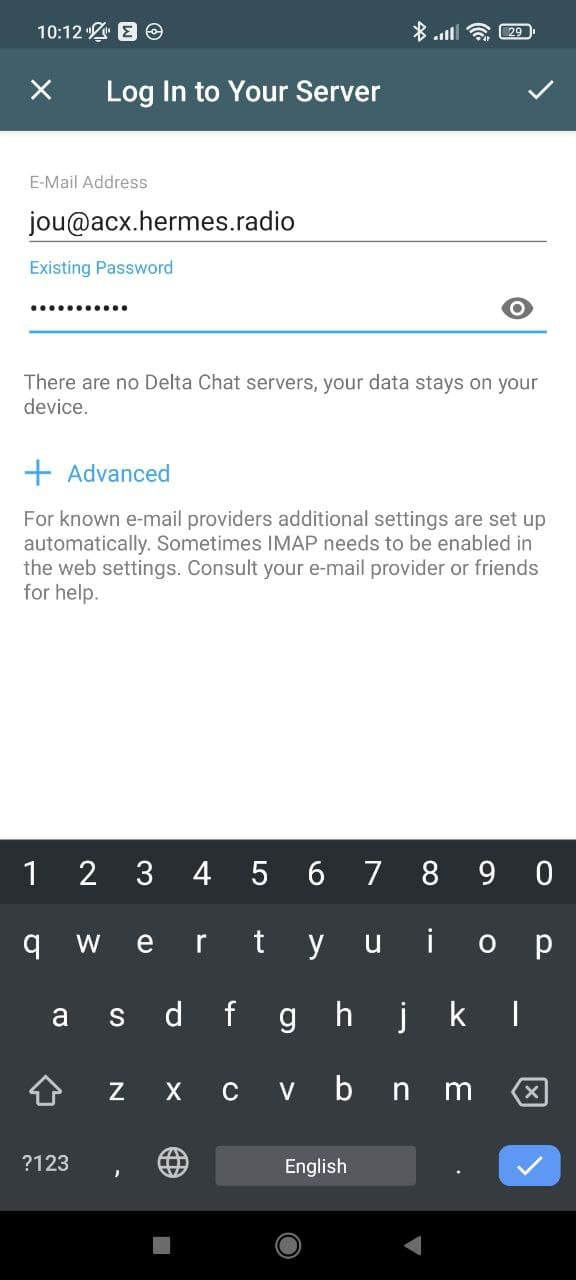
\includegraphics[width=0.3\columnwidth]{screenshots/deltachat/en/login.jpg}
    	\caption{Deltachat Login example}
	\vspace{-10pt}
    \label{fig:deltachat-login}
\end{figure}

% TODO: put DC pictures here
\subsection{Other email clients}
Other email clients can also be used. We can't cover all cases, but the HERMES system uses default services like IMAP to synchronize email folders and SMTP to send the messages. Specific technical information about the ports can be found in the appendix: \ref{apx_net_email}

\section{Troubleshooting}
The HERMES web interface indicates when something is wrong with the system. When a red dot appears in the footer bar (figure \ref{fig:status}), it becomes interactive, and when clicked, it lists the names of the services that are experiencing a problem.

\begin{figure}[H]
    \centering
    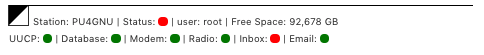
\includegraphics[width=0.8\columnwidth]{screenshots/frontend/en/status.png}
    	\caption{Red dot on the web interface can be clicked to check what part of the system may be broken}
    \label{fig:status}
\end{figure}

In case of problems with the antenna, a red led in the antenna (ANT) position will light up on the HERMES box (not the web interface). In this case, check the correct position of the power supply wires and check the position and integrity of the antenna, RF connectors, coaxial cable, and the transmitter. After checking that, it will be necessary to rest the antenna protection on the radio config section on the web interface for the radio transmit again. 

If the messages in the transmission list are not being transmitted at the allotted time, check that the radio settings have not been changed by going to the Admin tab. If that is not the case, it's possible that the other stations are offline.
%To remedy you could restore the factory default settings.



\pagebreak
\appendix{techinfo}
\label{techinfo}
\section{Appendix - technical information}
\subsection{Network Information}
\label{apx_net_info}

Each HERMES system provides a WiFi access point. The configuration is:
\begin{itemize}
\item WiFi Network Name: \texttt{HERMES}
\item WiFi Password: \texttt{amazonia}
\end{itemize}

The IP of the HERMES station (in the wireless interface) is \textbf{10.0.0.1} and the ethernet connection will connect as a dhcp client to an already existing network. 

%\item Server address: \url{hermes.radio} (IP \url{10.0.0.1})
\subsection{Network Services} 
\label{apx_net_services}

\subsubsection{E-mail services}
\label{apx_net_email}

The e-mail settings are the following:

\begin{itemize}
    \item Server address: \url{hermes} (IP \url{10.0.0.1})
    \item SMTP (Simple Mail Transfer Protocol): port \texttt{25}
    \item SMTPS (Secure Simple Mail Transfer Protocol): port \texttt{465}, with SSL support 
    (used for DeltaChat, the certificates are valid until 2031)
    \item IMAP (Internet Message Access Protocol): port \texttt{143}
    \item Webmail URL acessible: \url{http://hermen/mail} or \url{http://10.0.0.1/mail}
\end{itemize}

These settings should not be needed by most users as DeltaChat automatically identifies all the settings by entering just the e-mail address and password at the login prompt.

\subsubsection{Web services}
\label{apx_net_web}

The HERMES web interface runs on port 80 on http, and provides these capabilities:
\begin{itemize}
    \item BBS P2P public messaging capability (over UUCP);
    \item E-mail user administration;
    \item UUCP queue management;
    \item HF radio transceiver management tools;
    \item Customized permissions for users send multimedia messages;
    \item Page for radio service tasks (like test tone generation and PTT control);
    \item A network information page (for cases in which the HERMES system connects to a larger IP network);
    \item DeltaChat client downloads for Android, MacOS, Windows and Linux.
\end{itemize}

\subsection{Other network Services }
\label{apx_other_net}


\begin{itemize}
    \item SSH Secure Shell - for special system administration: port 22\newline
        \hfill user: "hermes", password: hermes\newline
        \hfill user: "root" password: "caduceu"
    \item VPN -  Virtual Private Network client ready for remote access
    %\item MQTT (Mosquitto server for network sensors integration's)
    \item ISPCONFIG admin web interface\newline
        \hfill port 8080 / credentials: "admin" "caduceu"
    \item mariaDB, the Database server for storing messages and users on station-api and ISPconfig
    \item E-mail services with transports connected to UUCP\newline
        \hfill Postfix, dovecot, spamassin, postgrey, amavis, clamav (hold) and ISPconfig as a manager 
    \item iwatch: handles inbox HMP folder and triggers UUCP spool compression
    \item hostapd: sets the wireless interface into Access Point mode
    \item dnsmasq: provides a domain name server and aliases 
    \item uucp: accessible via network with credentials user/pass%is this missing some info about user/password?
    \item VNC: Virtual X session environment with VARA monitor
        \hfill port: \texttt{5901} (Eg. in the local wifi network: vncviewer 10.0.0.1:5901) 
        \hfill user: "hermes", password: "hermes"
\end{itemize}

\section{Additional information}
\label{apx_adit_info}
    The main system runs Debian GNU/Linux release Bullseye and we try to follow their guidelines.

\subsection{Password Cheat Sheet}
\label{passwords}

% melhor duas tabelas? Uma para o Web, outra para WiFi?
% acho redundante, já tem as senhas nos serviços também
% isso é para ser um folheto separado
% para ser impresso várias vezes
% no manual, vamos colocar numa página sozinha, ao final
% (ou no começo...)
% junto com talvez outras informações básicas de como ligar e desligar a parada talvez
% ok, entao seria separado tipo um quick guide
% talvez seja melhor separar mesmo de arquivo e limpar as senhas daqui todas - pode ser, isso vai pro github

\begin{table}[h]

\centering
\begin{tabular}{|l|l|l|}
\hline
Description & User & Password  \\ \hline
Web Interface & root  & caduceu \\  \hline
WiFi Network & hermes & amazonia \\ \hline
\end{tabular}
\end{table}

\subsection{Field trials}
\label{apx_field_trials}
    HERMES system prototypes were tested on a test bed with stations installed in three cities: Brasília/DF, Belo Horizonte/MG and Hortolândia/SP. Most of the tests happened between Brasília and Belo Horizonte, and Belo Horizonte and Hortolândia. The straight line distance between Brasília and Belo Horizonte is 620 km, while Belo Horizonte and Hortolândia straight line distance is 470 km. All the stations are equipped with simple dipole installed as inverted V, tuned to the 40m amateur radio band.

    In our internal tests, between Belo Horizonte and Hortolândia, the modem reached more than 1000 bps in an average propagation condition (0db of SNR in the receiver). A 10Kb message, which is the typical size of an email with a picture takes about 4 minutes to be exchanged. In poor propagation conditions, this time can go up to 10 minutes. 

    The adaptive modem starts the communication with slower speeds, but if propagation is good, it gears up and automatically and increases the speed, and on the other hand, if propagation deteriorates, the modem reduces the speed, increasing the signal robustness.

\subsection{Source Code}
\label{apx_src}

    Source code is available inside the folders /home/hermen/install with the latest git versions before the deployment and is also available online at:
\begin{itemize}
    \item Web Front-end Interface, written using the Angular framework: \url{https://github.com/Rhizomatica/hermes-gui};
    \item Web Back-end Interface, written in PHP: \url{https://github.com/Rhizomatica/hermes-api}; 
    \item HF transceiver description and schematics: \url{https://github.com/DigitalHERMen/rhizo-transceiver};
    \item HF transceiver firmware and userland tools, written in C:
    \url{https://github.com/Rhizomatica/hermes-net};
    \item Network management software for UUCP and the HF modem (VARA or Ardop) integration, written in C:
    \url{https://github.com/DigitalHERMen/rhizo-uuardop}
\end{itemize}


\section{Licensing}
\label{apx_license}

    All the project's source code is licensed under the GPL version 3 or any greater version, unless stated differently in the repository.

\subsection{GNU General Public License Version 3}

    High-Frequency Emergency and Rural Multimedia Exchange System (HERMES).

    Copyright (C) 2021-2022 Rhizomatica.
\newline

    This program is free software: you can redistribute it and/or modify
    it under the terms of the GNU General Public License as published by
    the Free Software Foundation, either version 3 of the License, or
    (at your option) any later version.

    This program is distributed in the hope that it will be useful,
    but WITHOUT ANY WARRANTY; without even the implied warranty of
    MERCHANTABILITY or FITNESS FOR A PARTICULAR PURPOSE.  See the
    GNU General Public License for more details.

    You should have received a copy of the GNU General Public License
    along with this program.  If not, see <https://www.gnu.org/licensen/>.
    
\end{document}    
